\documentclass[12pt,epsfig]{article}
\usepackage{graphicx,fullpage,url}


\bibliographystyle{unsrt} %for BibTeX - sorted numerical labels by
                          %order of first citation.

\begin{document}

\pagestyle{empty}
\renewcommand{\thefootnote}{\fnsymbol{footnote}}

\begin{flushright}
{\small
Thomas Collins\\
NPG Technote \\ 
2019-TN-01\\
\today\\}
\end{flushright}

\vspace{.8cm}

\begin{center}
Methods for TEMPO-doping Araldite Epoxy\\   
\end{center}
\vspace{1cm}

\begin{abstract}
Araldite Epoxy doped with TEMPO has been found to be a suitable target material for dynamic nuclear polarization. Maximum proton polarization value of 13.8 percent has been achieved with a magnetic field of 4.998 T and a temperature of about 1.2 K. The simple process of preparing a TEMPO-doped target makes it an attractive option for DNP.      
\end{abstract}


%\tableofcontents

\section{Background/Motivation}

TEMPO-doped Araldite epoxy targets are attractive to DNP groups for their production properties. The targets are free form, quickly reproducible and relatively harmless in production. With simple machining of a teflon block you can create any shape for a target.   

\section{Safety}
Personal protective equipment while handling TEMPO.
\begin{enumerate}
\item Safety Mask 
\item Lab Coat
\item Gloves 
\item Eye Protection [Goggles]
\end{enumerate}
All TEMPO related activities must be performed under the fume hood. 

\section{Purpose}
This note is a generalized procedure for creating TEMPO-doped epoxy targets.

\subsection{List of Materials}
In the following, we describe a list of materials needed to make a TEMPO-doped epoxy target. 

List of Materials: 
\begin{enumerate}
\item  TEMPO
\item  Rapid (5min) Aralidte Epoxy 
\item  Magnet Wire
\item  Teflon (Polytetrafluoroethylene) Block 
\item  Teflon (Polytetrafluoroethylene) Sheet 
\end{enumerate}


\subsection{Procedure}
In the following, we  describe the  procedure. 

Procedure:
\begin{enumerate}
\item Prepare a Teflon mold suitable for your target cup. On one side of the mold create a channel large enough such that a coiled wire may pass through. 
\item Prepare a magnet wire coil such that its first loop is as large as possible while not in contact with any sides of the mold. Remaining wire must be coiled such that it fits through the channel prepared earlier.
\item Place teflon mold on teflon sheet inside fume hood. 
\item Place magnet wire coil inside the mold such that it is horizontal and suspended in the center of the mold. Cover the remainder of the channel so epoxy does not run out.  
\item Proper safety equipment must be worn from this point on. 
\item Thoroughly mix TEMPO and Resin. 1 part TEMPO for 100 part Resin. Place resin onto paper plate or any disposable surface, place TEMPO into resin and stir thoroughly for ~20sec or until TEMPO is uniformly distributed throughout the resin. Do not attempt to mix in plastic bag, this will led to an uneven mixture.    

ex.) 1mg TEMPO with 1g Resin. The Alpha target used in the Dec 2018 cooldown consisted of 6.98g Resin, 0.07-0.10g TEMPO, and 6.84g Hardener. [Inaccuracy in TEMPO due to scale fluctuations] 

\item Thoroughly mix TEMPO-Resin with Hardener. Amount of Hardener must equal the amount of Resin added in previous part. 1 part Resin with 1 part Hardener 

ex.) 1.001g TEMPO-Resin with 1g Hardener 
\item Pour TEMPO epoxy paste into teflon mold such that the coil is completely covered.
\item Let sit in fume hood until TEMPO epoxy fully cures. 
\item Remove TEMPO epoxy from mold. Clean excess from epoxy block so that it fits into target cup.
\item Safely store TEMPO epoxy target and clean fume hood, teflon block, and teflon sheet.
\end{enumerate}

\begin{figure}
\begin{center}
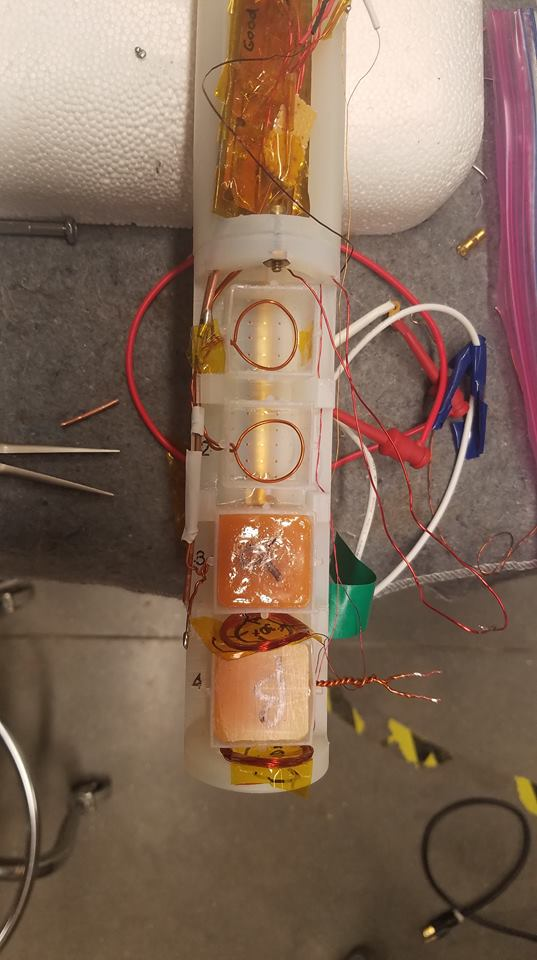
\includegraphics[angle=0,width=0.49\textwidth]{Target}
\caption{\label{ANCHOR} Target Stick with Alpha and Beta TEMPO Epoxy Targets}
\end{center}
\end{figure}

\begin{thebibliography}{2}
\bibitem{UVA} Yohei Noda, `Thermosetting polymer for dynamic nuclear polarization: Solidification of an epoxy resin mixture including TEMPO',Nuclear Instruments and Methods in Physics Research, 9 Dec 2014.
\end{thebibliography}


\end{document}

